\documentclass[9pt,twocolumn,twoside]{styles/osajnl}
\usepackage{fancyvrb}
\journal{i524} 

\title{Charge Detection Mass Spectrometry}

\author[1,*]{Scott McClary}

\affil[1]{School of Informatics and Computing, Bloomington, IN 47408, U.S.A.}

\affil[*]{Corresponding authors: scmcclar@indiana.edu}

\dates{project-001, \today}

\ociscodes{Chemistry, Cloud, HPC, I524, Parallel Computing}
\doi{\url{https://github.com/cloudmesh/sp17-i524/blob/master/project/S17-IO-3011/report/report.pdf}}

\begin{abstract}
A Charge Detection Mass Spectrometry research application is used to
show the benefits of using Ansible Galaxy. Previously, this
properitery research application was installed by hand on local
servers or Supercomputers. Transfering the input data to remote
systems as well as aggregating/visualizing the results is
difficult. Improving this research workflow by automating the
deoployment of the necessary software subsystems assists in building
an efficient, reproducible and scalable Charge Detection Mass
Spectrometry research workflow.
\newline
\end{abstract}

\setboolean{displaycopyright}{true}

\begin{document}

\maketitle

\section{Introduction} \label{introduction}
The Martin F. Jarrold research group studies Charge Detection Mass
Spectrometry. Their workflow consists of conducting scientific
experiments using a Mass Spectrometer. This instrument creates raw
data throughout each experiement. They have build an application a
Fast Fourier based application written in Fortran that processes the
output files to determine detailed mass information of the substance
used in the aformentioned experiment. The detailed mass information
outputted from the application can be used to solve important research
topics such as the measure of the the Hepatitis B virus, shown in figure
\ref{fig:hbvassembly}.

\begin{figure}
\centering
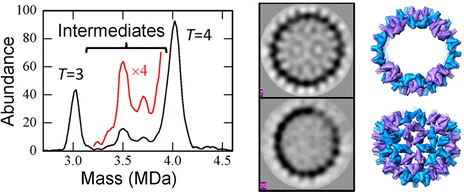
\includegraphics[height=1.35in, width=3.3in]{images/hbvassembly}
\caption{The chart to the left displays an accurate measurement of the Hepatitis B virus (HBV) created by the research group's CDMS application \cite{247}. This detailed mass information is used to create the images shown in the middle and to the right, which show 2-D and 3-D models of HBV.}
\label{fig:hbvassembly}
\end{figure}

\section{Execution Plan} \label{plan}
The following subsections act as a timeline regarding how I broke the
project up week-by-week in order to complete the entire project by the
desired deadline. The project execution plan is simply a guide and was
followed diligently; however, some items were pushed
forwards/backwards as technological challenges were faced.
\subsection{March 6, 2017 - March 12, 2017}
This week I installed Cloudmesh on my local machine, created my first
Virtual Machine on the Chameleon Cloud and tested Ansible Galaxy on
remote systems such as one or more Chameleon Cloud VM's. I also wrote
the project proposal, which will eventually become the project reoprt.
\subsection{March 13, 2017 - March 19, 2017}
This week I tested the deployment of the Intel Compiler on one or more
Chameleon Cloud VM's using Ansible Galaxy. I did not expect
significant progress to be made during this weeek given that I was out
of town for Spring Break.
\subsection{March 27, 2017 - April 2, 2017}
This week I deployed the Charge Detection Mass Spectrometry along with
the required input data on one or more Chameleon Cloud VM's using
Ansible Galaxy.
\subsection{April 3, 2017 - April 9, 2017}
This week I benchmarked both the deployment and the analysis on at
least one cloud (i.e. Chameleon Cloud). I also created a method to
aggregate the output from one or more VM's and locally visualize the
results.
\subsection{April 10, 2017 - April 16, 2017}
This week I wrote the majority of the project report. 
\subsection{April 17, 2017 - April 23, 2017}
This week I ensured the reproducibility of my source code as well as
revised the final version of the report.

\section{Ansible Galaxy} \label{licensing}
Ansible Galaxy was leveraged in order to automate the deoployment of
the required software subsystems, user code and data.

\subsection{Software Subsystems} \label{software}
The CDMS application relies on the Math Kernel Library (MKL) to
leverage efficient Fast Fourier Computations. The application also
leverages the OpenMP parallel framework in order to divide the work
amongst available CPU's. Therefore, in order to compile and run the
application, the Intel compiler is required, which provides the MKL
and OpenMP functionality.

\subsection{User Code} \label{code}
The Martin F. Jarrold Group has written a Fast Fourier Based
application written in Fortran in order to conduct their CDMS
research. This application is approximately 15,000 lines of
code. Depending on the input, about 60\% to 70\% of the compute time
is spent within external MKL libraries conducting FFT calculations.

\subsection{Data} \label{data}
The CDMS application inputs a set of raw 2 MB files. In order to
develop and test the efficiency of the deployment, a small and large
dataset was used. The small test dataset (i.e. 200 files) has a total
size of 400 MB and the large dataset (i.e. 4,506 files) has a total
size of 9.012 GB. A typical dataset for the research group is
approximately the size of the large dataset. In a single day, 7 to 10
datasets are created and need to be processed. When an algorithmic
change occurs to the research application, a large batch of archived
data requires reprocessing. In this case, terabytes of data may be
processed. This is why the parallelization and therefore the
scalability of the application is critical to the Martin F. Jarrold
research group.

\section{CDMS Research Pipeline} \label{cdms}
\begin{figure}
\centering
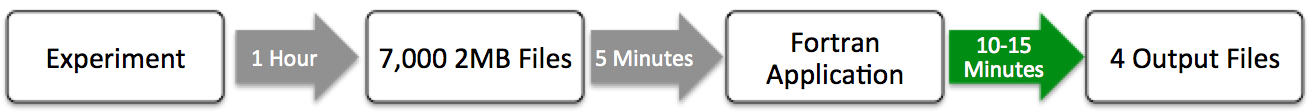
\includegraphics[height=0.45in, width=3.3in]{images/pipeline}
\caption{CDMS Pipeline}
\end{figure}

\section{Licensing} \label{licensing}
TBD

\section{Benchmark}
As discussed in section \ref{code}, the application is parallelized
using OpenMP. Therefore, this application utilizes the avaialable
computational power available. Figure \ref{fig:scalability2} compares the performance of the application on difference compute resources (i.e. local servers, Supercomputers and clouds). 

The time required to deploy and run the application in the cloud is
shown in the figure (TBD). This benchmark includes the time required
for the installation of the software subsystems as well as the time
required to run the application. 

\subsection{OpenMP Scalability} \label{scalability}
\begin{figure}
\centering
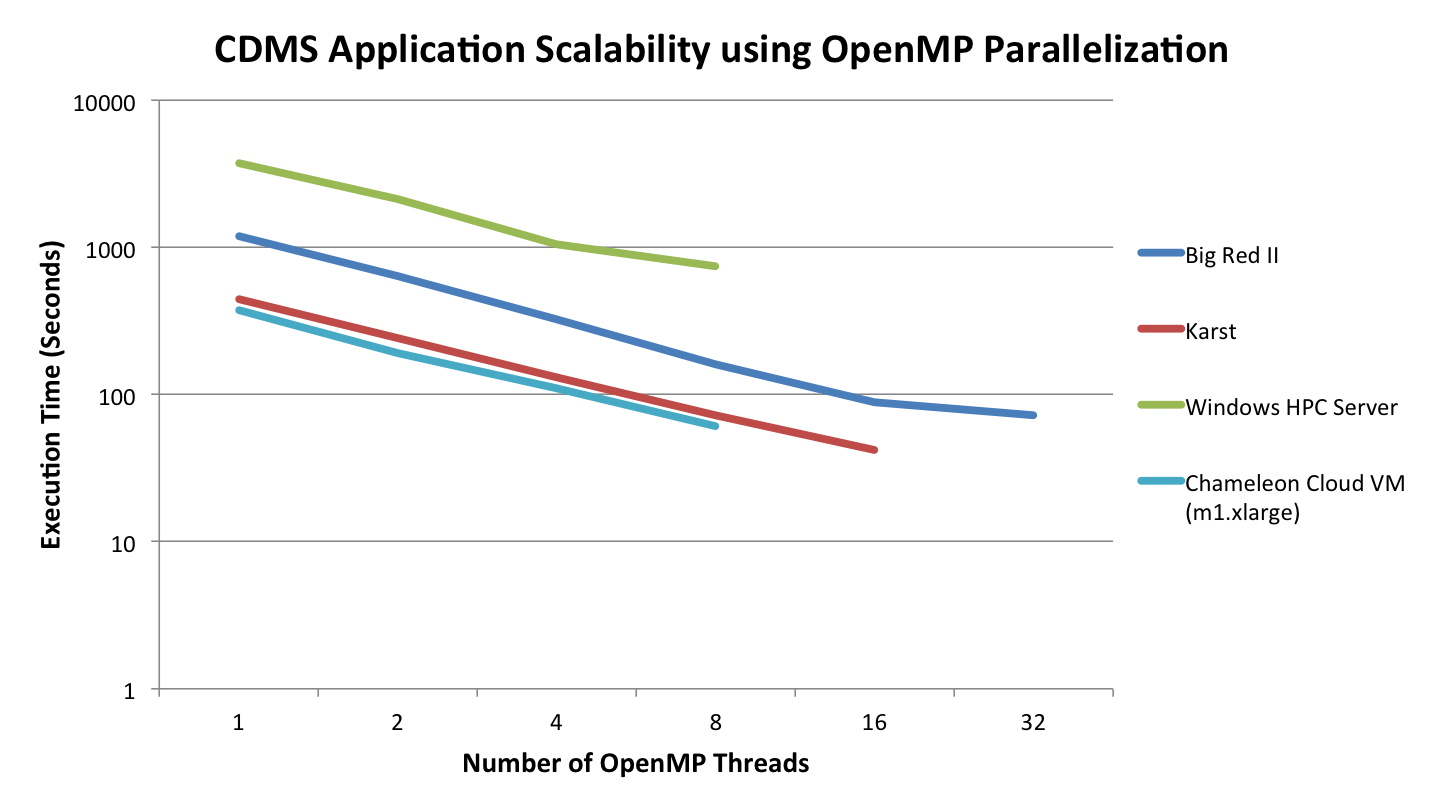
\includegraphics[height=2.3in, width=3.3in]{images/scalability2}
\caption{The figure above shows the scalability (i.e. reduction in time-to-solution) as the number of OpenMP threads increase on local servers, Supercomputers and Clouds.}
\label{fig:scalability2}
\end{figure}

\section{Conclusion} \label{conclusion}
The use of Ansible Galaxy to run the Charge Detection Mass
Spectrometry application in the Cloud (e.g. Chameleon Cloud) imporved
the efficiency, reproduciblity and scalability. In comparison to
running on the Indiana University HPC clusters (e.g. Karst and Big Red
II), the application time-to-solution diminished sigificantly. The
most important and useful tool that was developped as a result of this
project was the automation of the deployment of the necessary software
subsystems, the application itself, the necessary input data and
aggregation/visualization of the output. The use of Ansible Galaxy
within this research workflow will allow the Martin F. Jarrold
research group to focus on the details of their specific research
rather than on the details of managing the software subsystems,
running the application and managing the input/output data.

\section*{Acknowledgements}
The authors would like to thank the School of Informatics and
Computing for providing the Big Data Software and Projects (INFO-I524)
course \cite{www-i524}. This project would not have been possible
without the technical support \& edification from Gregor von Laszewski
and his distinguished colleagues.

 
\section*{Author Biographies}
\begingroup
\setlength\intextsep{0pt}
\begin{minipage}[t][3.2cm][t]{1.0\columnwidth} 
  \begin{wrapfigure}{L}{0.25\columnwidth}
    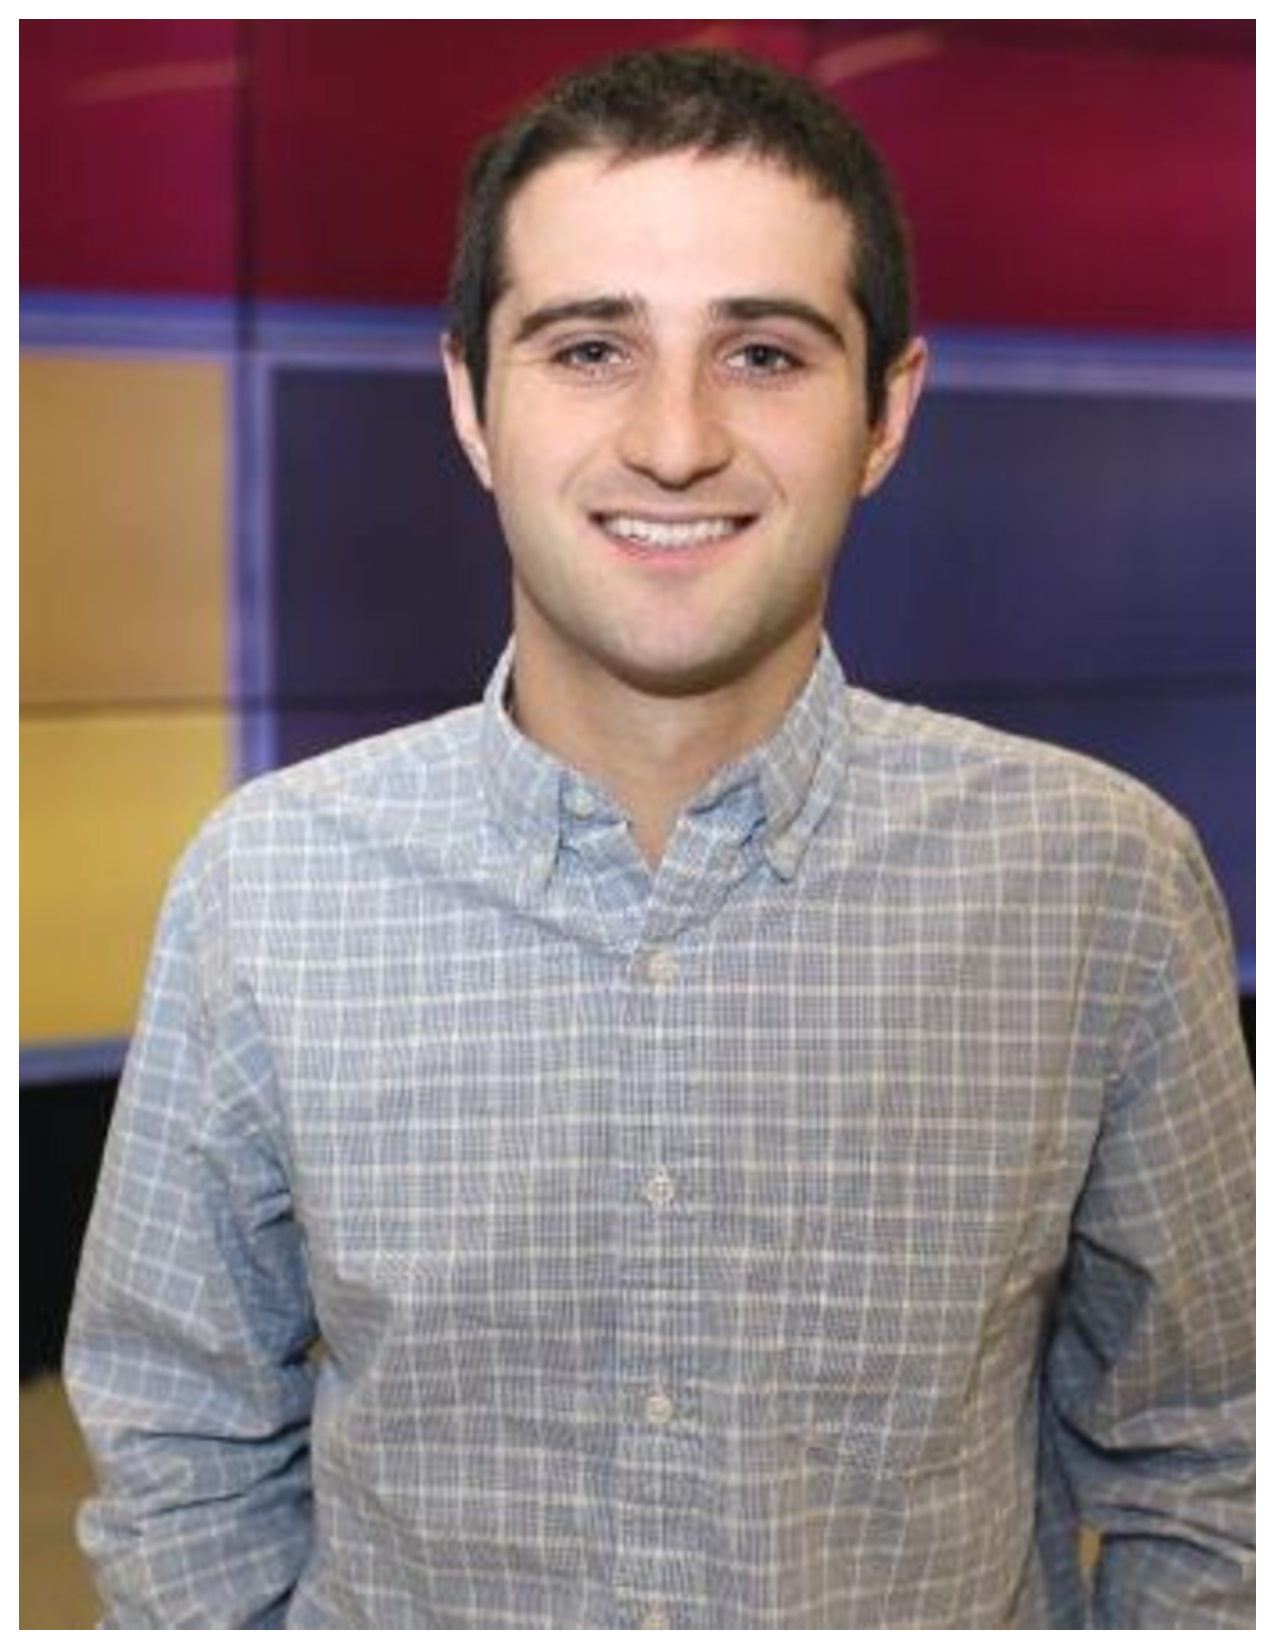
\includegraphics[width=0.25\columnwidth]{images/scott_mcclary}
  \end{wrapfigure}
  \noindent
  {\bfseries Scott McClary} received his BSc (Computer Science) and
  Minor (Mathematics) in May 2016 from Indiana University and will
  receive his MSc (Computer Science) in May 2017 from Indiana
  University. His research interests are within scientific application
  performance analysis on large-scale HPC systems. He will begin
  working as a Software Engineer with General Electric Digital in San
  Ramon, CA in July 2017.
\end{minipage}
\endgroup

\section*{} %used to create more spacing..
\section*{Work Breakdown}
The work on this project was distributed as follows between the
authors:
\begin{description}
\item[Scott McClary.] He completed all of the work for this paper
  including researching and testing Apache Airavata as well as
  composing this technology paper.
\end{description}

% Bibliography
\bibliography{references}
\end{document}

